\documentclass[10pt]{article}
\usepackage[utf8]{inputenc}
\usepackage{listings}
\usepackage{float}
\usepackage{graphicx}
\usepackage{fullpage}
\usepackage{caption}
\usepackage{subcaption}
\usepackage{amsmath}
\usepackage{hyperref}
\usepackage{epstopdf}
\usepackage{csvsimple}

%\renewcommand{\thesubsection}{\arabic{subsection}}
\renewcommand{\thesubsubsection}{\alph{subsubsection}}

\title{Pattern Recognition Practical 6}
\author{Group 24: \and Maikel Withagen (s1867733) \and Steven Bosch (s1861948)}
\date{\today}
\lstset{
frame=single, 
numbers=left, 
breaklines=true, 
language=Matlab,
basicstyle=\footnotesize, 
title=\lstname,
showstringspaces=false
}

\DeclareMathOperator*{\argmax}{arg\!\max}

\renewcommand{\thesection}{Assignment \arabic{section}}
\renewcommand{\thesubsection}{\arabic{subsection}}
\begin{document}
\maketitle

\section{}
\subsection{}
When we take $k=2$ the Minkowski metric is the same as the Euclidean distance between the points, which is used as error function in other clustering methods such as K-means clustering.

\subsection{}
See section \ref{Minkowski} in the appendix for our implementation.

\subsection{}
Looking at figure \ref{fig1a} we can clearly distinguish four main clusters within the data. The figures show that for higher values of t more connections are plotted. This is logical since a higher threshold permits higher distances between two points to be plotted, which overall results in more plotted connections. As for the optimal value of t, 0.05 is clearly too low, because we can see some connections within the clusters, but a lot of points that clearly belong to the clusters are left out because their distance to the other points is too high (see figure \ref{fig1b}). We can still see this for a t of 0.1, but on a smaller scale (see figure \ref{fig1c}). On the other hand a t of 0.25 is clearly too high, because multiple different clusters get connected through outliers, causing multiple clusters to be clustered together (see figure \ref{fig1f}). The same thing happens with a t of 0.2, where the two left clusters are connected (see figure \ref{fig1e}). Since this does not happen for a t of 0.15 and almost all of the points are assigned to a cluster (see figure \ref{fig1d}), this seems to be the optimal value of t. There is one point that does not get assigned to a cluster, so we will have to accept this as an outlier that does not belong to any cluster. 

\begin{figure}[H]
  \centering
  \caption{Minkowski clustering for different threshold values.}
	\begin{subfigure}[b]{.49\textwidth}
		\includegraphics[width=\columnwidth]{Ass1_0.eps}
		\caption{}
		\label{fig1a}
	\end{subfigure}  
	\begin{subfigure}[b]{.49\textwidth}
		\includegraphics[width=\columnwidth]{Ass1_5.eps}
		\caption{}
		\label{fig1b}
	\end{subfigure}
	\quad
	\begin{subfigure}[b]{.49\textwidth}
		\includegraphics[width=\columnwidth]{Ass1_10.eps}
		\caption{}
		\label{fig1c}
	\end{subfigure}
	\begin{subfigure}[b]{.49\textwidth}
	   	\includegraphics[width=\columnwidth]{Ass1_15.eps}
	   	\caption{}
	   	\label{fig1d}
	\end{subfigure}
	\quad
	\begin{subfigure}[b]{.49\textwidth}
	   	\includegraphics[width=\columnwidth]{Ass1_20.eps}
	   	\caption{}
	   	\label{fig1e}
	\end{subfigure}
	\begin{subfigure}[b]{.49\textwidth}
		\includegraphics[width=\columnwidth]{Ass1_25.eps}
		\caption{}
		\label{fig1f}
	\end{subfigure}	
  \label{fig1.1}
\end{figure}

\section{}
\subsection{}
See section \ref{Ass2} in the appendix for our implementation.
\begin{figure}
	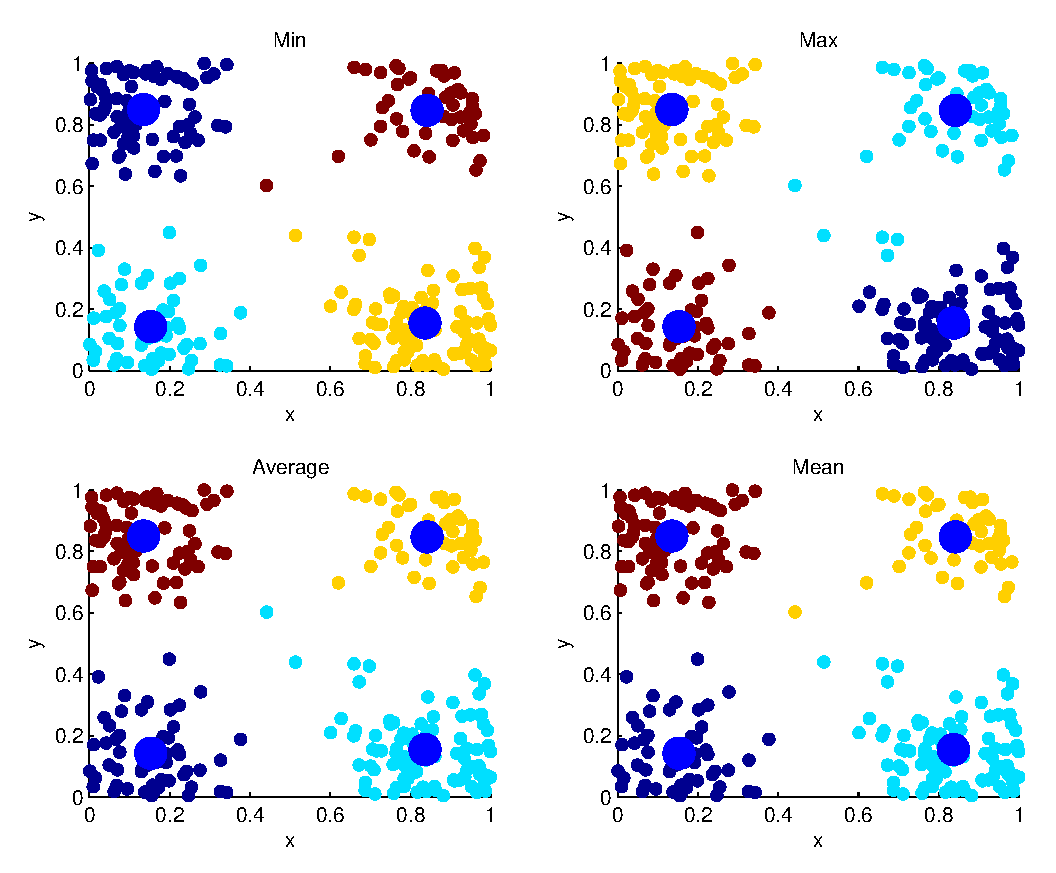
\includegraphics[width=\columnwidth]{Ass2_1.eps}
	\caption{Agglomerative hierarchical clustering using different distance functions. The big circles are the centroids per cluster.}
	\label{fig2a}
\end{figure}
Figure \ref{fig2a} shows the different clusterings the agglomerative hierarchical clustering method yields for different distances. As we can see, the different distances yield similar clusters but not entirely equal. The data points that are in the middle of the graphs get attributed to different clusters, dependening on the distance type used. When we interpret the different clusterings by just looking at the plots, it seems like the minimum and the mean distance yield the best solutions out of the four. But to know for certain an error could be computed to see which distance yields the best results.

\subsection{}
\begin{figure}
	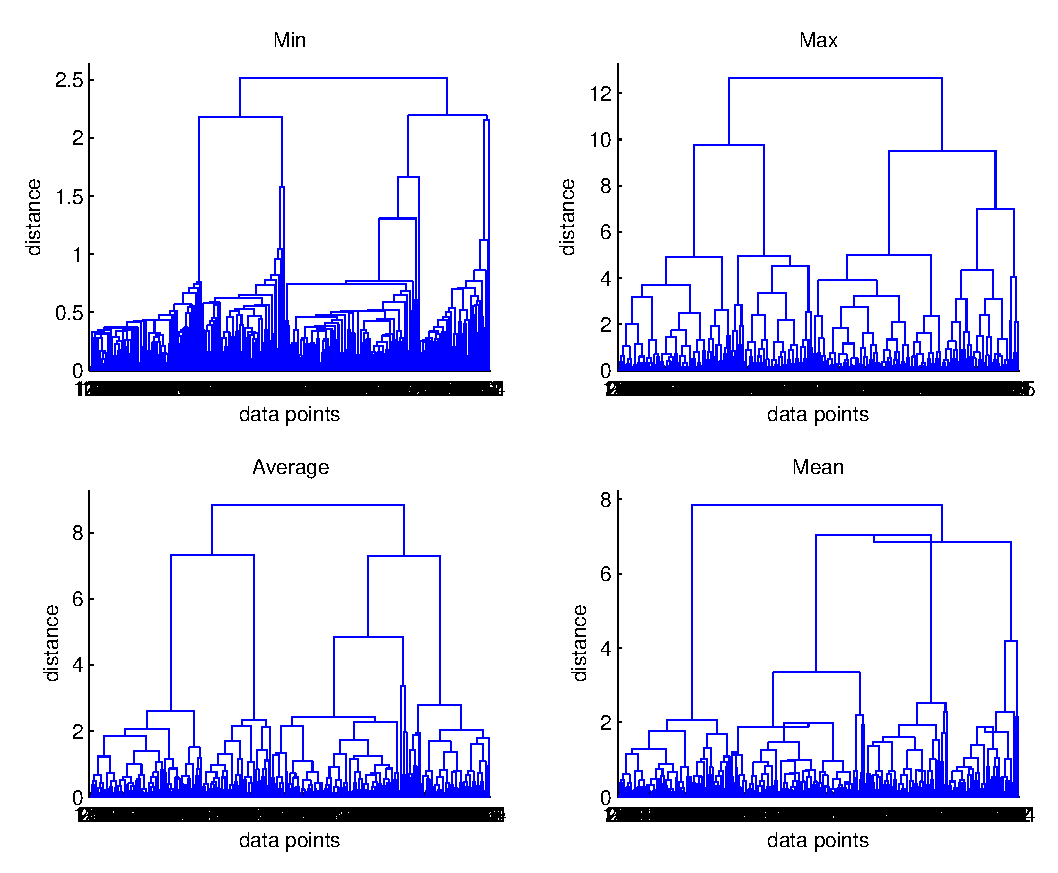
\includegraphics[width=\columnwidth]{Ass2_2.eps}
	\caption{Dendroids for the agglomerative hierarchical clustering using different distance functions.}
	\label{fig2b}
\end{figure}
Figure \ref{fig2b} gives the dendograms for the agglomerative hierarchical clustering using different distance functions. Let us assume four main clusters again. We can extrapolate information about the distances between members of these four clusters from these graphs. For example, the minimum distance dendogram shows us the minimum distances between members of the four main clusters: the nearest members of the first two main clusters shown in the graph (from left to right) lie about 0.75 units apart, whereas the nearest members of the last two main clusters lie very close (in the order of 0.05 units) to each other. The nearest members between the first two clusters and the last two clusters are about 0.25 units apart. 

Similarly we can deduce from the maximum distance graph that the farthest members from the first two main clusters lie about 5 units apart and from the last two main clusters about 3 units. Between the first and last two clusters the farthest members lie about 3 units apart. The average member of the first two clusters lie about 4 units apart and those of the last two clusters about 2 units. The average members between the first and last two clusters lie about 2 units apart.

Finally in the mean graph we can see something different with respect to the previous three. Here the centroid of one cluster is farther away from the three other clusters than their centroids are to each other. So there is one cluster that lies further apart from the other three, whereas the previous three graphs did not show that. This is probably due to the fact the last method uses distances between centroids, which is more robust towards outliers than the other three methods. Therefore the first three graphs do not show this, while the last one does.

\section{}
\subsection{}
Using the code given in section \ref{Ass3} in the appendix, we computed the J-values for the different clusterings, shown in figure \ref{tab1}
\begin{table}[H]
	\centering
	\caption{$J_e$-values for different clusters}
	\label{tab1}
	\begin{tabular}{c|c}
		Clustering & $J_e$ \\
		\hline
		$\{\{x1, x2, x3\}, \{x4, x5\}\}$ & 13.1667\\
		$\{\{x2, x3, x5\}, \{x1, x4\}\}$ & 20.6667\\
		$\{\{x4\}, \{x1, x2, x3, x5\}\}$ & 17.7500\\
		$\{\{x4, x5\}, \{x1, x2, x3\}\}$ & 13.1667\\
		$\{\{x3, x5\}, \{x1, x2, x4\}\}$ & 22.6667
	\end{tabular}
\end{table}

\subsection{}
Table \ref{tab1} shows that the clusterings $\{\{x1, x2, x3\}, \{x4, x5\}\}$ and $\{\{x4, x5\}, \{x1, x2, x3\}\}$ minimize the sum-of-squared error. The order of the clusters does not matter (different orderings of a sum yield the same result), as long as they have the same members. That is why these two clusterings yield the same result. 

\section{}
Table \ref{tab4} shows the dissimilarity matrix of the z-transformed data on the twelve provinces in the Netherlands. Figures \ref{fig4a}, \ref{fig4b} and \ref{fig4c} show dendrograms for the data using single linkage (minimum distance) clustering. Let us first look at the first dendrogram, which shows the clustering for all features combined. The dendrogram shows two main clusters and one outlier, South Holland. The first cluster is made up out of Gelderland, North Brabant and North Holland, the second out of the rest. We see that especially the provinces of Flevoland, Limburg, Zeeland, Overijssel, Drenthe and Friesland are close to each other, with Friesland and Drenthe being the closest (0.64 dissimilarity). The most different provinces overall are Flevoland and South Holland (dissimilarity of 5.72).

Looking at the other dendrograms we can explain parts of these results. Especially population seems to have a big impact. South Holland is the most distance away from all of the other clusters. We can see in the data: South Holland has by far the highest population, followed by North Holland, North Brabant and Gelderland, three provinces that get clustered together. All of the other provinces get clustered together as well, although within that cluster we can see a clear distinction between the smaller clusters Overijssel, Limburg and Utrecht, and Drenthe, Friesland, Groningen, Zeeland and Flevoland, the latter having the lowest populations. So populations seems to have a large contribution to the overall clustering.

Area seems to have some effect as well. The provinces seem to be scattered more over the clusters, but at least one aspect does contribute: Gelderland and North Brabant show a clear distinction from the other provinces (they are much larger), so this contributes to the overall clustering in which these two provinces are clustered together. 

Density seems to have a large effect on the overall (all features) clustering, since we see much similar clustering here. Again Limburg, Overijssel, Drenthe, Friesland, Zeeland, Groningen and Flevoland are clustered into one group. There are some extra members though (Gelderland and North Brabant) and one member (Utrecht) is now in another cluster, but we see a lot of similarity, indicating that density has a large contribution on the overall clustering. 

Looking at the GDP dendrogram we can see that South Holland again is not clustered together with other provinces. It's GDP differs by a large degree to the other provinces. Combined with the population difference we saw earlier this explains why South Holland is also an outlier in the main clustering with all the features combined. We also see here that North Brabant and North Holland are immediately combined into one cluster (because they have the exact same GDP: 65.295), which partly explains why they are relatively close in the main clustering. Furthermore we again see a lot of the same provinces close to each other.

Finally the GDP per cap shows that North Brabant and North Holland are again immediately combined, because they have the same GDP per cap.\footnote{NB This is curious, since they do have the same GDP but not the same population.} Also we see Drenthe and Friesland very close to each other, just like in the main clustering.

Overall we see a lot of similar trends in many of features, which was of course to be expected. The dendrograms show some interesting aspects. For example, Gelderland and North Brabant are mostly clustered together because of their area and population. In the other features they differ quite much, but apparently there was just no other province or cluster of provinces that came closer. From the dendrograms we can also deduce some relationships between features. We see that there is a strong relation between population and GDP, which is logical because more people often earn more together than fewer people. Furthermore it looks like there is a relation between population and GDP per cap. This can be explained by the fact that most people move towards areas where they have the perspective of earning the most.

\begin{table}
	\centering
	\caption{The dissimilarity matrix of the z-transformed data on the twelve provinces in the Netherlands.}
	\label{tab4}
	\resizebox{\textwidth}{!}{\csvautotabular{dissMatrixAss4.csv}}
\end{table}

\begin{figure}
	\includegraphics[width=\columnwidth]{Ass4a.eps}
	\caption{Dendroids for the agglomerative hierarchical clustering of the provinces using different distance functions.}
	\label{fig4a}
\end{figure}
\begin{figure}
	\includegraphics[width=\columnwidth]{Ass4b.eps}
	\caption{Dendroids for the agglomerative hierarchical clustering of the provinces using different distance functions.}
	\label{fig4b}
\end{figure}
\begin{figure}
	\includegraphics[width=\columnwidth]{Ass4c.eps}
	\caption{Dendroids for the agglomerative hierarchical clustering of the provinces using different distance functions.}
	\label{fig4c}
\end{figure}

\newpage
\section*{Appendix}
\appendix
\section{Assignment 1}
\lstinputlisting{../Code/Ass1.m}{\label{Minkowski}}
\section{Assignment 2}
\lstinputlisting{../Code/Ass2.m}{\label{Ass2}}
\section{Assignment 3}
\lstinputlisting{../Code/Ass3.m}{\label{Ass3}}
\section{Assignment 4}
\lstinputlisting{../Code/Ass4.m}{\label{Ass4}}

\end{document}
